\documentclass{sig-alternate-ipsn09}

\usepackage{graphicx}
\usepackage{times}
\usepackage{epsfig}
\usepackage{psfrag}
\usepackage{amssymb}
\usepackage{amsmath}
\usepackage{mathenv}
\usepackage{epstopdf}
%\usepackage{algorithmic}
%\usepackage{algorithm}

\usepackage{fancyhdr}


\begin{document}

\title{A Sample {\ttlit ACM} SIG Proceedings Paper in LaTeX
Format\titlenote{(Does NOT produce the permission block, copyright information nor page numbering). Supported by ACM.}}
%
% You need the command \numberofauthors to handle the 'placement
% and alignment' of the authors beneath the title.
%
% For aesthetic reasons, we recommend 'three authors at a time'
% i.e. three 'name/affiliation blocks' be placed beneath the title.
%
% NOTE: You are NOT restricted in how many 'rows' of
% "name/affiliations" may appear. We just ask that you restrict
% the number of 'columns' to three.
%
% Because of the available 'opening page real-estate'
% we ask you to refrain from putting more than six authors
% (two rows with three columns) beneath the article title.
% More than six makes the first-page appear very cluttered indeed.
%
% Use the \alignauthor commands to handle the names
% and affiliations for an 'aesthetic maximum' of six authors.
% Add names, affiliations, addresses for
% the seventh etc. author(s) as the argument for the
% \additionalauthors command.
% These 'additional authors' will be output/set for you
% without further effort on your part as the last section in
% the body of your article BEFORE References or any Appendices.

\numberofauthors{8} %  in this sample file, there are a *total*
% of EIGHT authors. SIX appear on the 'first-page' (for formatting
% reasons) and the remaining two appear in the \additionalauthors section.
%
\author{
% You can go ahead and credit any number of authors here,
% e.g. one 'row of three' or two rows (consisting of one row of three
% and a second row of one, two or three).
%
% The command \alignauthor (no curly braces needed) should
% precede each author name, affiliation/snail-mail address and
% e-mail address. Additionally, tag each line of
% affiliation/address with \affaddr, and tag the
% e-mail address with \email.
%
% 1st. author
\alignauthor
Ben Trovato\titlenote{Dr.~Trovato insisted his name be first.}\\
       \affaddr{Institute for Clarity in Documentation}\\
       \affaddr{1932 Wallamaloo Lane}\\
       \affaddr{Wallamaloo, New Zealand}\\
       \email{trovato@corporation.com}
% 2nd. author
\alignauthor
G.K.M. Tobin\titlenote{The secretary disavows
any knowledge of this author's actions.}\\
       \affaddr{Institute for Clarity in Documentation}\\
       \affaddr{P.O. Box 1212}\\
       \affaddr{Dublin, Ohio 43017-6221}\\
       \email{webmaster@marysville-ohio.com}
% 3rd. author
\alignauthor Lars Th{\o}rv{\"a}ld\titlenote{This author is the
one who did all the really hard work.}\\
       \affaddr{The Th{\o}rv{\"a}ld Group}\\
       \affaddr{1 Th{\o}rv{\"a}ld Circle}\\
       \affaddr{Hekla, Iceland}\\
       \email{larst@affiliation.org}
\and  % use '\and' if you need 'another row' of author names
% 4th. author
\alignauthor Lawrence P. Leipuner\\
       \affaddr{Brookhaven Laboratories}\\
       \affaddr{Brookhaven National Lab}\\
       \affaddr{P.O. Box 5000}\\
       \email{lleipuner@researchlabs.org}
% 5th. author
\alignauthor Sean Fogarty\\
       \affaddr{NASA Ames Research Center}\\
       \affaddr{Moffett Field}\\
       \affaddr{California 94035}\\
       \email{fogartys@amesres.org}
% 6th. author
\alignauthor Charles Palmer\\
       \affaddr{Palmer Research Laboratories}\\
       \affaddr{8600 Datapoint Drive}\\
       \affaddr{San Antonio, Texas 78229}\\
       \email{cpalmer@prl.com}
}
% There's nothing stopping you putting the seventh, eighth, etc.
% author on the opening page (as the 'third row') but we ask,
% for aesthetic reasons that you place these 'additional authors'
% in the \additional authors block, viz.
\additionalauthors{Additional authors: John Smith (The Th{\o}rv{\"a}ld Group,
email: {\texttt{jsmith@affiliation.org}}) and Julius P.~Kumquat
(The Kumquat Consortium, email: {\texttt{jpkumquat@consortium.net}}).}
\date{30 July 1999}
% Just remember to make sure that the TOTAL number of authors
% is the number that will appear on the first page PLUS the
% number that will appear in the \additionalauthors section.

%Sections go here.  An example of figures is shown in Figure~\ref{fig:example}.
%\begin{figure}
%\centering
%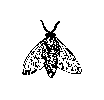
\epsfig{file=fly.eps}
%\caption{A sample black and white graphic (.eps format).}
%\label{fig:example}
%\end{figure}


\maketitle
\begin{abstract}
\label{sec:abstract}

Cyber-Physical Systems (CPS) consist of computational components interconnected by computer networks that monitor and control switched physical entities interconnected by physical infrastructures. To ensure a tight integration among the components in CPS we employ a novel approach that composes the correctness of components instead of their functionality using conjunction of non-interfering logical invariants. Our distributed algorithm developed for smart power grid nodes uses this approach to adaptively schedule power migrations in such a way that the stability of both the computer network and the physical system are maintained. In this paper we mainly focus on network congestion and explore a well known Explicit Congestion Notification (ECN) scheme from CPS context and demonstrate the significant improvement in overall CPS efficiency and stability. Experimentation results show how the power transfers between smart grid nodes are unaffected if nodes are allowed to exploit ECN scheme while also taking necessary actions to reduce network congestion.
\end{abstract}

\section{Introduction}
\label{sec:introduction}

Smart Power Grid~\cite{huang11} is a prime example of Cyber-Physical System 
(CPS) where the goal is to have embedded computing devices monitor and control 
distributed generation, storage and transfer of power in a safe, reliable, 
efficient and secure manner. Ensuring stability and correctness (both logical and temporal)
of the system as a whole is a major challenge in CPS design. Any incorrectness or 
instability in one component can impact the same features of other components. 
For example, an action in the physical domain could affect the network domain and 
vice-versa, thus making correct scheduling of these actions paramount to overall system
stability. The fundamental challenge in developing a design framework that
unifies the various components is the heterogeneity of the component types,
resulting in semantic gaps that must be bridged. 

% comparison
Existing papers largely consider the stability of one or two components in
isolation. For example, network delays affect system stability and considerable
work focusses on determining system stability bounds as a function of injected
delay~\cite{hespanha07}. Results from switched-systems theory~\cite{donkers11}
model the stability of the plant. Hybrid automata~\cite{henzinger96} and timed
I/O automata~\cite{alur94} represent a simultaneous mix of continuous and
discrete states in the verification process~\cite{chutinan03,tomlin03}.
Real-time scheduling is traditionally a function of \emph{a priori} time
bounds~\cite{liu00}. To consider components individually, or in pairs, requires
that they be very stable such that the composition of the components into a CPS
is stable.

In our work, we employ a fundamentally different approach that composes
correctness instead of functionality. The basic idea, depicted in
Figure~\ref{fig:invariant_conjunction}, is to express the stability and
correctness constraints of all components in the form of logical {\em invariants} 
and ensure that system actions are performed only if and when they are guaranteed not 
to violate the conjunction of these invariants. This approach is not only limited
to smart power grid design but can also be generalized to different cyber-physical systems 
with different functionalities. 

\begin{figure}[htb]
  \begin{center}
%    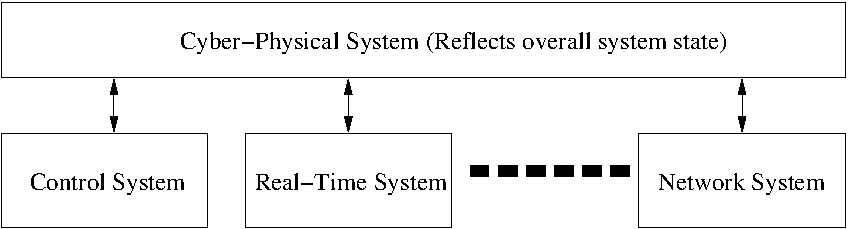
\includegraphics[width=0.45\textwidth]{Figures/cps-n-domains.pdf}
     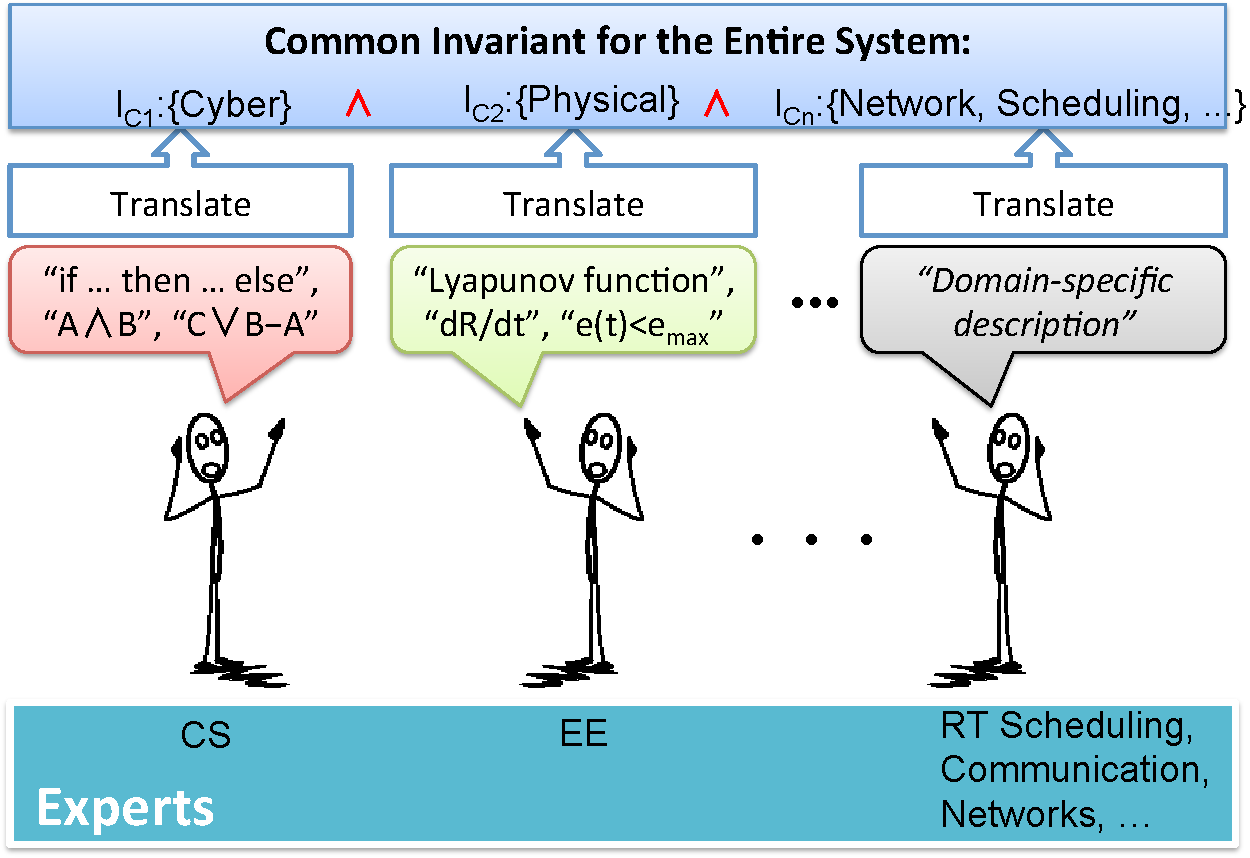
\includegraphics[width=0.9\columnwidth]{Figures/Invariant_Overview.pdf}
  \caption{Overview of invariant-based approach}
  \label{fig:invariant_conjunction}
  \end{center}
\end{figure}

The state of the physical system and, hence, its stability, is dependent on
power transfers (series of power migrations) initiated by the cyber algorithm
within each node in the system and by the state of the communication network
that carries messages between the cyber nodes to signal initiation and
acknowledgement of physical power migrations. The state and stability of the
communication network is in turn affected by the number of migration messages in
transit at any given time. In recent work[*****cite COMPSAC], we developed a 
scheduling invariant for our distributed, adaptive algorithm for scheduling power 
migrations between nodes in a smart grid and demonstrate that conjunction of such a
scheduling invariant and an invariant for physical system state is necessary to 
maintain overall system stability. In contrast to traditional real-time scheduling, 
{\em correct} scheduling in our context refers to initiating actions at appropriate 
times in a way that system stability is maintained rather than insisting that every 
action is initiated at a pre-defined time and must adhere to a pre-defined deadline. 
In order to improve efficiency along with stability, components in CPS must have 
certain amount of inter-component information. In the current paper, we focus on 
improving the efficiency while also maintaining the stability of smart grid nodes 
by exploiting the network congestion information obtained from Early Congestion 
Notification (ECN) scheme, wherein packets are marked indicating impending congestion,
instead of dropping them\cite{floyd1994tcp, ramakrishnan1999proposal, 
ramakrishnan2001addition}. We allow the smart grid nodes to sense the possible 
upcoming network congestion and change the amount of power being transferred with 
every power migrate message in order to compensate for reduced rate of power transfers.
As of our knowledge, this is the first work that explore ECN scheme from CPS context
for the benefit of physical system efficiency as well as take necessary action to 
reduce network congestion.

The rest of this paper is organized as follows. Section \ref{sec:related_work}
provides some background information and discusses related work. We present our
system model and assumptions in Section \ref{sec:assumptions}. Section
\ref{sec:invariants} presents our physical system 
invariant and adaptive scheduling invariant. Section \ref{sec:power_management_algo} 
presents our resulting power management algorithm. Our simulation setup is introduced 
in Section \ref{sec:simulation_setup} and results are presented in Section
\ref{sec:results}. Section \ref{sec:discussion} presents a brief discussion and
conclusions are presented in Section \ref{sec:conclusions}.



\section{Background and Related Work}
\label{sec:related_work}

Most of the Cyber-physical systems are switched, continuous time dynamic systems with changes occurring at discrete time intervals~\cite{liberzon03}. Analyzing CPS is a complicated task, as it consists of tight coupling of various components that are heterogeneous in nature, such as, cyber,  physical and network. In CPS, actions performed in one component should not affect the stability in another components. Therefore, it is mandatory to schedule \textit{correct} actions at \textit{correct} time in each component of CPS in order to maintain overall system stability. However, only stability and correct scheduling is not enough, the system should also be adaptive in nature when uncertain components are present in the composed CPS. Typically, most of the CPS kind of applications, involve communication network as one of the important components ("smart grid" as a prime example). Standalone physical systems with computational capability, such as power plants, vehicular systems, medical devices, and robotics - just to name few - have been deeply studied in the literature, but when these kind of systems are interconnected through unreliable or uncertain communication network, like internet, physical system aspects, assumptions, control strategies and functional behavior is affected due to the unpredictability of transmission time in the communication network. 

A verification technique for Cyber-Physical systems was recently proposed in~\cite{DAC_2012_CPS_verification} assuming communication network to be CAN, FlexRay. etc, wherein authors use structured properties of network infrastructures and efficiently bound network delays. 
In~\cite{SmartGridLoadScheduling}, authors propose an idea of scheduling power demands for optimal energy management in smart-grid, but they do not consider the network behavior. In traditional real-time systems, dynamic adaptation is normally performed at "sporadic intervals" using elastic scheduling techniques~\cite{Buttazzo_IEEE_Jornl_2002} and feedback scheduling~\cite{FeedbackScheduling07}, but CPS requires continuous adaptation. Adaptive scheduling proposed in ~\cite{AdaptiveScheduling_DASC_1999}, dynamically changes the task execution rate based on the observed system behavior, but requires complete abstraction of physical and network parameters. Similar approach can be taken to dynamically change the power transfer rate across the smart-grid nodes based on the observed network conditions, but abstraction of internet like network parameters (eg. RTT, Round-Trip time) is non-trivial. In our recent paper~\cite{acsmartgrid}, we proposed an adaptive algorithm which schedules power migrate messages between CPS smart-grid nodes based on the observed round-trip times in internet like network. This algorithm forms invariant which in conjunction with physical system invariant achieves stability of the overall system. The main reason of unpredictable round-trip times (in internet) is the nature of the traffic, increase in traffic might lead to exponential increase in transmission delays and can also cause messages to drop.

[******add citations]
{\bf Protocols for CPS,} although internet protocols such as TCP are well known for reliability, TCP relies on packet drops caused due to overflow of queues at gateways as an indication of network congestion. 
In smart grid context, every message is responsible for a small amount of power in the
grid, therefore a loss of message is directly associated to the grid stability. TCP by controlling 
its transmission rate can effectively reduce packet drops if transport is capable of ECN.
But, congestion information obtained from network is completely hidden from the application
running over TCP. In order to know ECN in application, User Datagram Protocol (UDP) is a perfect choice.
It is then application's responsibility to adapt according to network conditions and take 
necessary actions upon detection of congestion in the network.
[******end citations]



%\section{System Model And Assumptions}
\label{sec:assumptions}

{\bf Power Management Architecture.} Figure~\ref{fig:SmartGridArchi-fig} shows
the architecture of a future generation smart grid (SmartGrid)~\cite{huang11}.
The system is essentially a microgrid consisting of energy storage devices
(DESD), energy resources (DRER) and LOADs. Each node is potentially owned and
located in a residence or business and the basic idea is to share power among
nodes in order to benefit the overall system. Intelligent flow controllers
(nodes) contain Solid State Transformers (SSTs), that are physical actuators
controlling power flow to and from a shared electrical bus under the direction
of co-operating Distributed Grid Intelligence (DGI) processes.

The DGI processes are cyber algorithms that choose, negotiate and manage power
transfers among nodes based on local information and information about the
states of other nodes that is periodically exchanged among nodes. In the current
work, we assume that all nodes are synchronized, for the sake of simplicity.
Nodes periodically exchange state information with each other in a state
collection phase. Next, a negotiation phase is performed in which nodes conduct
negotiations to identify which power transfers need to be performed among nodes.
The identified power transfers between pairs of nodes are then performed in a
power transfer phase. One cycle is depicted in Figure\ref{fig:cycle}, with one
or more negotiation and power transfer phase pairs after a state collection
phase. This entire cycle of state collection, negotiation and power transfer
phases is repeated.

\begin{figure}[htb]
  \begin{center}
    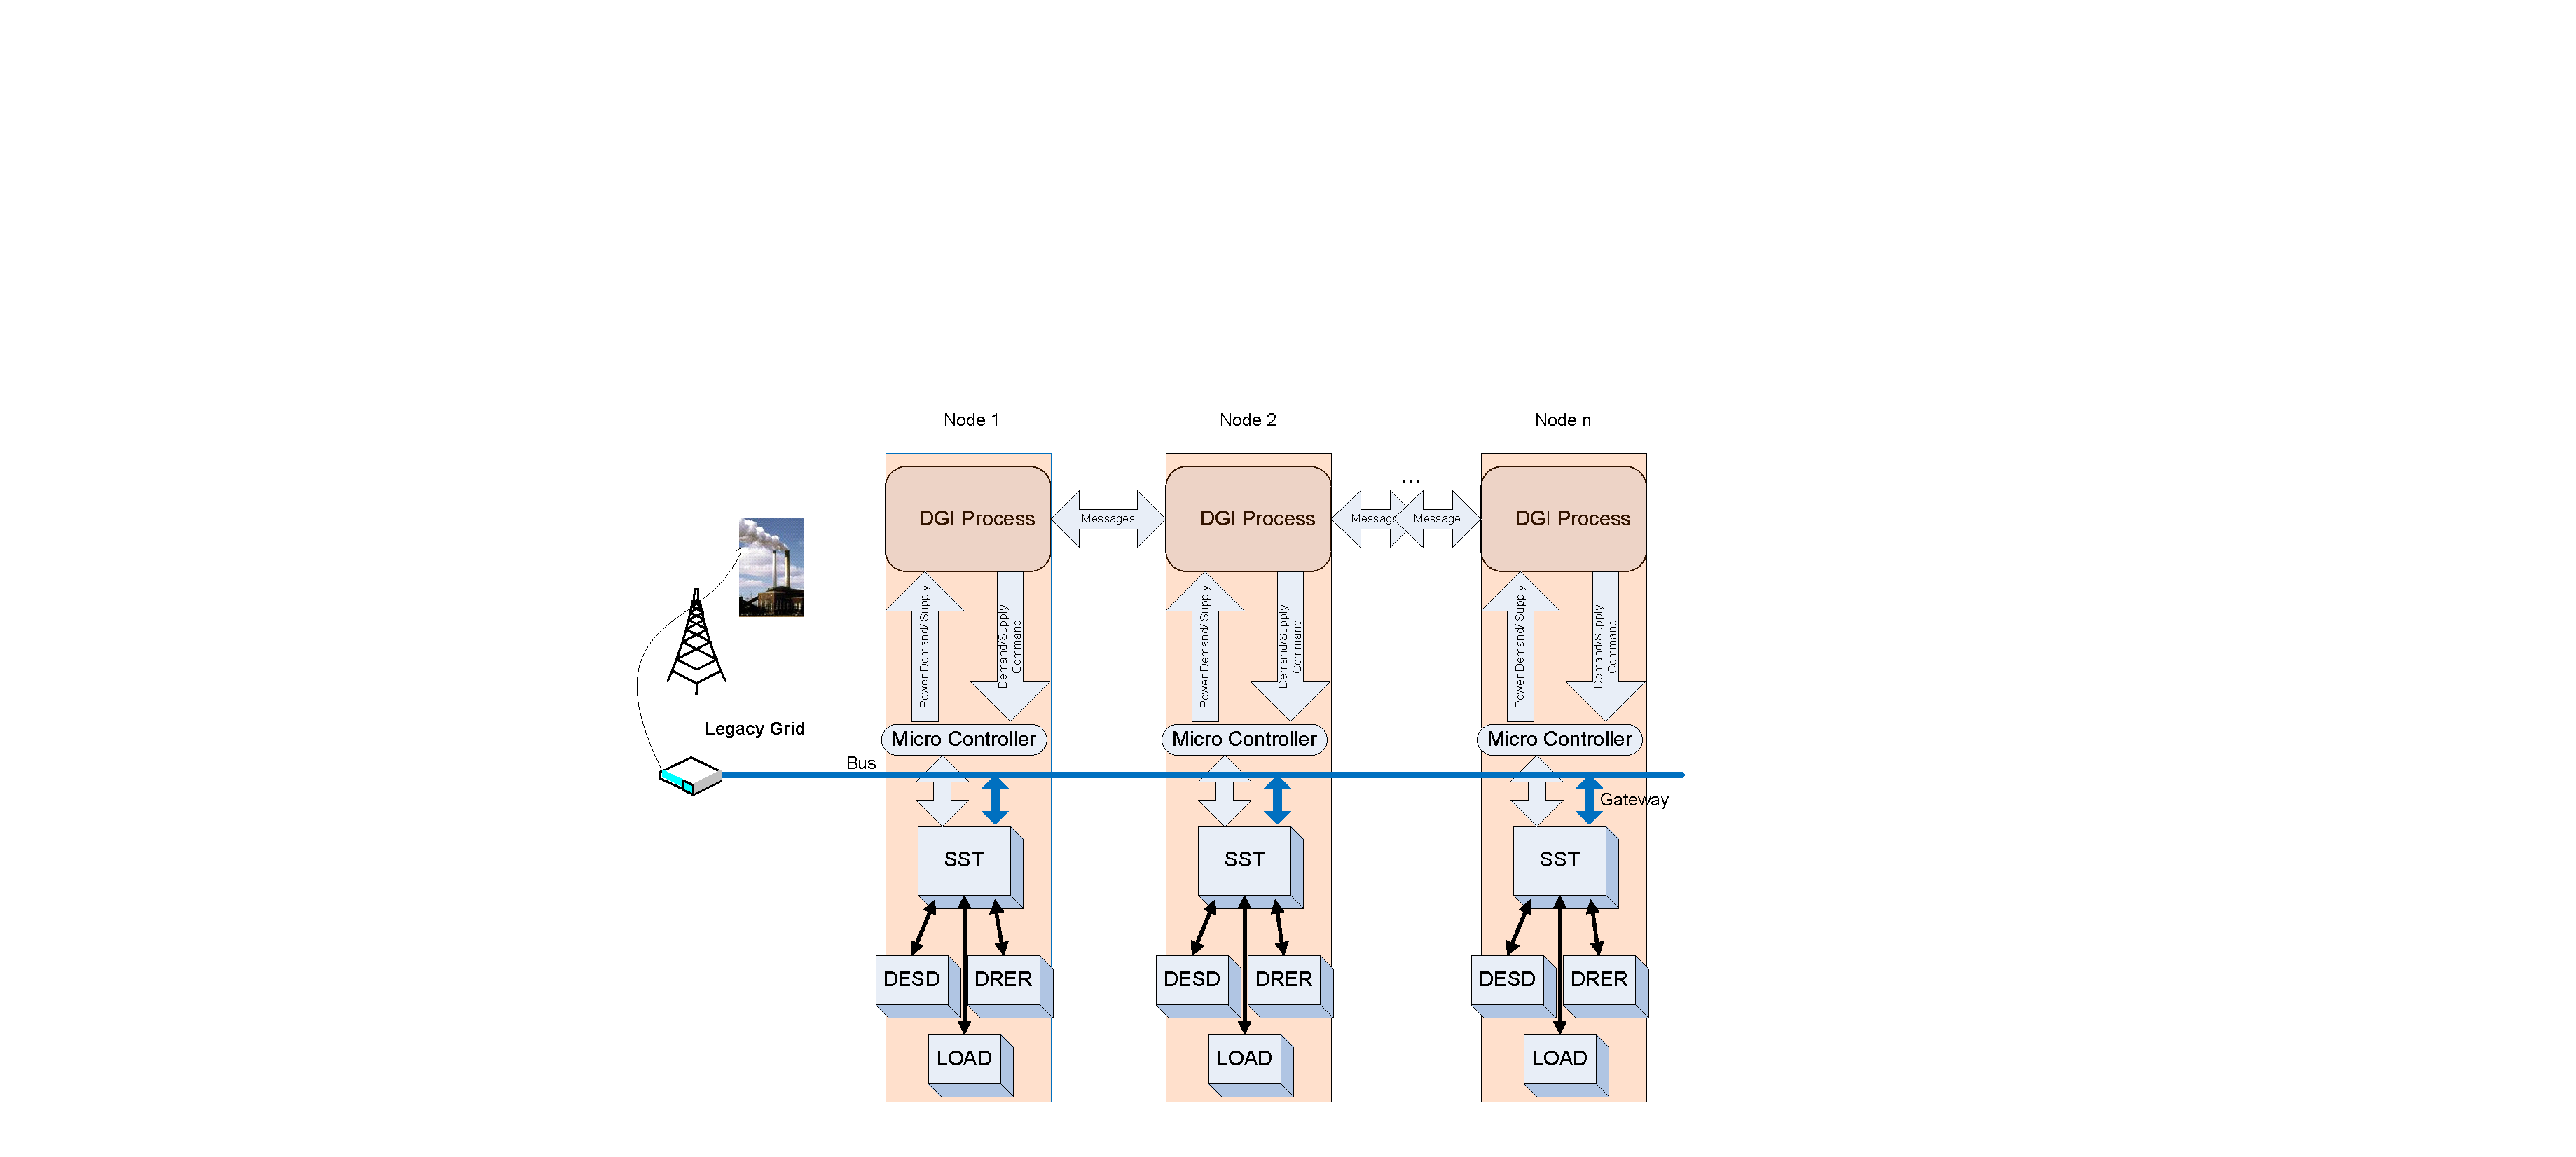
\includegraphics[width=0.45\textwidth]{Figures/DistributedLoadBalancing3.pdf}
  \caption{Smart Grid Power Management Architecture}
  \label{fig:SmartGridArchi-fig}
  \end{center}
\end{figure}

\begin{figure}[htb]
  \begin{center}
    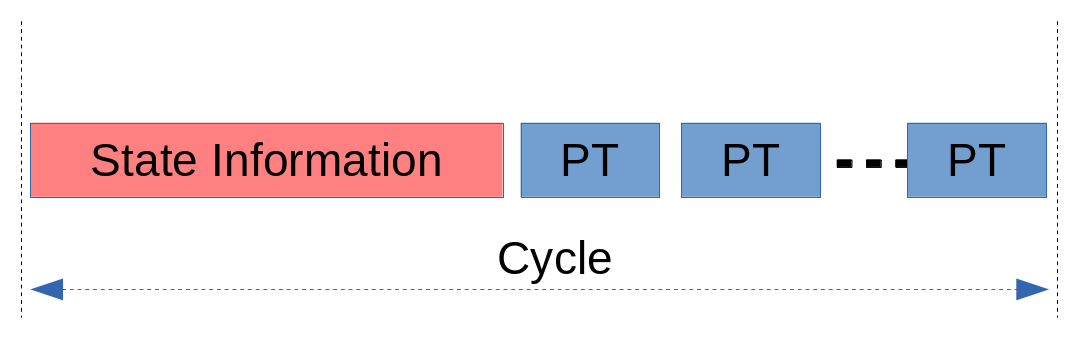
\includegraphics[width=0.45\textwidth]{Figures/cycle_fig.png}
  \caption{A single cycle of collecting state information followed by many negotiation and power transfer phases (PT)}
  \label{fig:cycle}
  \end{center}
\end{figure}

{\bf Power Transfer Model.} Power transfers within one phase are performed as a
series of (periodic) power migrations, each transferring a given quantum (say
$\delta$) of power. The cyber algorithm on the source (sender) node sends
appropriate control signals to the local physical actuators to add a quantum of
power to the electrical bus and sends a power migration message to the
destination (receiver) node signaling this. Upon receiving this power migration
message, the destination node sends control signals to its local physical
actuators to remove a quantum of power from the electrical bus and sends an
acknowledgement message to the source node.

{\bf Physical System Model.} The physical system is a finite inertia microgrid,
that is, a power system with a small number of generators and loads that acts
independently of the grid. There is a relatively small rotating generator,
whose inertia dominates the dynamics as described in the next section. There
are some number of controllable nodes that participate in the power management
by acting as either loads or generators. Nodes with excess generating capacity
transfer power to nodes that have excess load.

{\bf Communication Model.} 
Each node in the network runs an adaptive message scheduling algorithm that schedules power migrate messages in any given 
topology, based on the observed communication latencies at a given node. 


%\input{physicalsystem}

%\input{networksystem}

\section{Methodology}
Methodology goes here


\section{Conclusions}
Conclusion goes here.

%ACKNOWLEDGMENTS are optional
\section*{Acknowledgments}
Acknowledgement goes here.

%
% The following two commands are all you need in the
% initial runs of your .tex file to
% produce the bibliography for the citations in your paper.
\bibliographystyle{abbrv}
\bibliography{sigproc}  % sigproc.bib is the name of the Bibliography in this case
% You must have a proper ".bib" file
%  and remember to run:
% latex bibtex latex latex
% to resolve all references

\begin{thebibliography}{10}

\setlength{\itemsep}{-0.01mm}
\footnotesize

\bibitem{cyphy}
{IEEE} workshop on design, modeling and evaluation of cyber physical systems.

\bibitem{omnet}
The {OMNeT}++ discrete event simulation system.

\bibitem{aikat2003variability}
J.~Aikat, J.~Kaur, F.~Smith, and K.~Jeffay.
\newblock Variability in tcp round-trip times.
\newblock In {\em Internet Measurement Conference: Proceedings of the 3 rd ACM
  SIGCOMM conference on Internet measurement}, volume~27, pages 279--284, 2003.

\bibitem{5622003}
R.~Akella, F.~Meng, D.~Ditch, B.~McMillin, and M.~Crow.
\newblock Distributed power balancing for the freedm system.
\newblock In {\em Smart Grid Communications (SmartGridComm), 2010 First IEEE
  International Conference on}, pages 7 --12, October 2010.

\bibitem{alur94}
R.~Alur and D.~L. Dill.
\newblock A theory of timed automata.
\newblock {\em Theoretical Computer Science}, 126(2):183--235, 1994.

\bibitem{Bak2010}
S.~Bak, A.~Greer, and S.~Mitra.
\newblock Hybrid cyberphysical system verification with simplex using discrete
  abstractions.
\newblock In {\em Real-Time and Embedded Technology and Applications Symposium
  (RTAS), 2010 16th IEEE}, pages 143 --152, april 2010.

\bibitem{5587717}
S.~Bensalem, A.~Legay, T.-H. Nguyen, J.~Sifakis, and R.~Yan.
\newblock Incremental invariant generation for compositional design.
\newblock In {\em Theoretical Aspects of Software Engineering (TASE), 2010 4th
  IEEE International Symposium on}, pages 157 --167, aug. 2010.

\bibitem{GarlanKrogh2010}
A.~Bhave, B.~Krogh, D.~Garlan, and B.~Schmerl.
\newblock Multi-domain modeling of cyber-physical systems using architectural
  views.
\newblock In {\em Proceedings of the 1st Analytic Virtual Integration of
  Cyber-Physical Systems Workshop.}, 30 November 2010.
\newblock Co-located with RTSS 2010.

\bibitem{branicky98}
M.~S. Branicky.
\newblock Multiple lyapunov functions and other analysis tools for switched and
  hybrid systems.
\newblock {\em IEEE Transactions on Automatic Control}, 43(4):475--482, 1998.

\bibitem{Buttazzo_IEEE_Jornl_2002}
G.~Buttazzo, G.~Lipari, M.~Caccamo, and L.~Abeni.
\newblock Elastic scheduling for flexible workload management.
\newblock {\em Computers, IEEE Transactions on}, 51(3):289 --302, mar 2002.

\bibitem{chutinan03}
A.~Chutinan and B.~H. Krogh.
\newblock Computational techniques for hybrid system verification.
\newblock {\em IEEE Transactions on Automatic Control}, 48:64--75, January
  2003.

\bibitem{Alfaro}
L.~de~Alfaro and M.~Stoelinga.
\newblock Interfaces: A game-theoretic framework to reason about open systems.
\newblock In {\em FOCLASA 03: Proceedings of the 2nd International Workshop on
  Foundations of Coordination Languages and Software Architectures, Electronic
  Notes on Theoretical Computer Science}. Elsevier Science Publishers, 2003.

\bibitem{DerlerLeeSangiovanniVincentelli12_ModelingCyberPhysicalSystems}
P.~Derler, E.~A. Lee, and A.~Sangiovanni-Vincentelli.
\newblock Modeling cyber-physical systems.
\newblock {\em Proceedings of the IEEE (special issue on CPS)}, 100(1):13 --
  28, January 2012.

\bibitem{AdaptiveScheduling_DASC_1999}
B.~Doerr, T.~Venturella, R.~Jha, C.~Gill, and D.~Schmidt.
\newblock Adaptive scheduling for real-time, embedded information systems.
\newblock In {\em Digital Avionics Systems Conference, 1999. Proceedings.
  18th}, volume 1/17 pp. vol.1, pages 2.D.5--1 --2.D.5--9 vol.1, nov 1999.

\bibitem{donkers11}
M.~C.~F. Donkers, W.~P. M.~H. Heemels, N.~van~de Wouw, and L.~Hetel.
\newblock Stability analysis of networked control systems using a switched
  linear systems approach.
\newblock {\em IEEE Transactions on Automatic Control}, 56:2101--2115, 2011.

\bibitem{floyd1994tcp}
S.~Floyd.
\newblock Tcp and explicit congestion notification.
\newblock {\em ACM SIGCOMM Computer Communication Review}, 24(5):8--23, 1994.

\bibitem{guo2003bayesian}
D.~Guo and X.~Wang.
\newblock Bayesian inference of network loss and delay characteristics with
  applications to tcp performance prediction.
\newblock {\em Signal Processing, IEEE Transactions on}, 51(8):2205--2218,
  2003.

\bibitem{henia_ernst_rtss_2007}
R.~Henia and R.~Ernst.
\newblock Scenario aware analysis for complex event models and distributed
  systems.
\newblock In {\em IEEE Real-Time Systems Symposium}, pages 171--180, Los
  Alamitos, CA, USA, 2007.

\bibitem{henzinger96}
T.~A. Henzinger.
\newblock The theory of hybrid automata.
\newblock In {\em IEEE Symposium on Logic in Computer Science}, pages 278--292,
  1996.

\bibitem{hespanha07}
J.~P. Hespanha, P.~Naghshtabrizi, and Y.~Xu.
\newblock A survey of recent results in networked control systems.
\newblock {\em Proceedings of the IEEE}, 95:138--162, 2007.

\bibitem{Hoare85}
C.~Hoare.
\newblock {\em Communicating Sequential Processes}.
\newblock Prentice Hall, 1985.

\bibitem{hollot2001control}
C.~Hollot, V.~Misra, D.~Towsley, and W.~Gong.
\newblock A control theoretic analysis of red.
\newblock In {\em INFOCOM 2001. Twentieth Annual Joint Conference of the IEEE
  Computer and Communications Societies. Proceedings. IEEE}, volume~3, pages
  1510--1519. IEEE, 2001.

\bibitem{huang11}
A.~Q. Huang, M.~L. Crow, G.~T. Heydt, J.~P. Zheng, and S.~J. Dale.
\newblock {The Future Renewable Electric Energy Delivery and Management
  (FREEDM) System: The energy internet}.
\newblock {\em Proceedings of the IEEE}, 99(1):133--148, Jan. 2011.

\bibitem{jiang2002passive}
H.~Jiang and C.~Dovrolis.
\newblock Passive estimation of tcp round-trip times.
\newblock {\em ACM SIGCOMM Computer Communication Review}, 32(3):75--88, 2002.

\bibitem{SmartGridLoadScheduling}
I.~Koutsopoulos and L.~Tassiulas.
\newblock Control and optimization meet the smart power grid: scheduling of
  power demands for optimal energy management.
\newblock In {\em Proceedings of the 2nd International Conference on
  Energy-Efficient Computing and Networking}, e-Energy '11, pages 41--50, 2011.

\bibitem{DAC_2012_CPS_verification}
P.~Kumar, D.~Goswami, S.~Chakraborty, A.~Annaswamy, K.~Lampka, and L.~Thiele.
\newblock A hybrid approach to cyber-physical systems verification.
\newblock In {\em 49th ACM/EDAC/IEEE Design Automation Conference (DAC)}, pages
  688 --696, june 2012.

\newpage

\bibitem{ReconfigurationCBSECRTST2012}
P.~Kumar, N.~Stoimenov, and L.~Thiele.
\newblock An algorithm for online reconfiguration of resource reservations for
  hard real-time systems.
\newblock In {\em ECRTS}, pages 245--254, 2012.

\bibitem{liberzon03}
D.~Liberzon.
\newblock {\em Switching in Systems and Control}.
\newblock Birkhauser, Boston, 2003.

\bibitem{liu00}
J.~Liu.
\newblock {\em Real-Time Systems}.
\newblock Prentice Hall, 2000.

\bibitem{martin2000analysis}
H.~Martin, A.~McGregor, and J.~Cleary.
\newblock Analysis of internet delay times.
\newblock {\em Measurement}, 2000.

\bibitem{OwickiGries1976}
S.~Owicki and D.~Gries.
\newblock An axiomatic proof technique for parallel programs.
\newblock {\em Acta Informatica}, 6:319--340, 1976.

\bibitem{paul12thesis}
T.~Paul.
\newblock {\em Unified Knowledge Model for Stability Analysis in Cyber Physical
  Systems}.
\newblock Missouri University of Science and Technology, 2012.

\bibitem{paul2011}
T.~Paul, J.~Kimball, M.~Zawodniok, T.~Roth, and B.~McMillin.
\newblock Invariants as a unified knowledge model for cyber-physical systems.
\newblock In {\em Service-Oriented Computing and Applications (SOCA), 2011 IEEE
  International Conference on}, pages 1 --8, dec. 2011.



\bibitem{pei2009passive}
Y.~Pei, H.~Wang, and S.~Cheng.
\newblock A passive method to estimate tcp round trip time from nonsender-side.
\newblock In {\em Computer Science and Information Technology, 2009. ICCSIT
  2009. 2nd IEEE International Conference on}, pages 43--47. IEEE, 2009.



\bibitem{quet2002guidelines}
P.~Quet, S.~Chellappan, A.~Durresi, M.~Sridharan, H.~{\"O}zbay, and R.~Jain.
\newblock Guidelines for optimizing multi-level ecn, using fluid flow based tcp
  model.
\newblock {\em Proc. ITCOM-2002}, pages 106--116, 2002.

%\newpage

\bibitem{ramakrishnan1999proposal}
K.~Ramakrishnan and S.~Floyd.
\newblock A proposal to add explicit congestion notification (ecn) to ip.
\newblock Technical report, RFC 2481, January, 1999.

\bibitem{ramakrishnan2001addition}
K.~Ramakrishnan, S.~Floyd, D.~Black, et~al.
\newblock The addition of explicit congestion notification (ecn) to ip, 2001.

\bibitem{real_crespo_rts_2004}
J.~Real and A.~Crespo.
\newblock Mode change protocols for real-time systems: A survey and a new
  proposal.
\newblock {\em Real-Time Systems}, 26(2):161--197, 2004.

\bibitem{sha_rts_1989}
L.~Sha, R.~Rajkumar, J.~Lehoczky, , and K.~Ramamritham.
\newblock Mode change protocols for priority-driven preemptive scheduling.
\newblock {\em Real-Time Systems}, 1(3):243--264, 1989.

\bibitem{shakkottai2004rtt}
S.~Shakkottai, R.~Srikant, N.~Brownlee, A.~Broido, et~al.
\newblock The rtt distribution of tcp flows in the internet and its impact on
  tcp-based flow control.
\newblock 2004.

\bibitem{DBLP:SitzoffG93}
M.~Sintzoff and F.~Geurts.
\newblock Analysis of dynamical systems using predicate transformers -
  attraction and composition.
\newblock In {\em Analysis of Dynamical and Cognitive Systems}, pages 227--260,
  1993.

\bibitem{stoimenov_date_2009}
N.~Stoimenov, S.~Perathoner, and L.~Thiele.
\newblock Reliable mode changes in real-time systems with fixed priority or edf
  scheduling.
\newblock In {\em Design, Automation and Test in Europe}, pages 99--104. IEEE,
  April 2009.

\bibitem{tomlin03}
C.~J. Tomlin, I.~Mitchell, A.~M. Bayen, and M.~Oishi.
\newblock Computational techniques for the verification of hybrid systems.
\newblock {\em Proceedings of the IEEE}, 91:986--1001, July 2003.

\bibitem{omnetpaper}
A.~Varga.
\newblock The omnet++ discrete event simulation system.
\newblock {\em Proceedings of the European Simulation Multiconference
  (ESM'2001)}, June 2001.

\bibitem{FeedbackScheduling07}
F.~Xia, G.~Tian, and Y.~Sun.
\newblock Feedback scheduling: an event-driven paradigm.
\newblock {\em SIGPLAN Not.}, 42(12):7--14, Dec. 2007.

\bibitem{ye98impulse}
H.~Ye, A.~N. Michel, and L.~Hou.
\newblock Stability analysis of systems with impulse effects.
\newblock {\em IEEE Transactions on Automatic Control}, 43(12):1719--1723,
  1998.

\bibitem{ye98hybrid}
H.~Ye, A.~N. Michel, and L.~Hou.
\newblock Stability theory for hybrid dynamical systems.
\newblock {\em IEEE Transactions on Automatic Control}, 43(4):461--474, 1998.

\bibitem{Zhu:2010:MEE:1795194.1795196}
Y.~Zhu, E.~Westbrook, J.~Inoue, A.~Chapoutot, C.~Salama, M.~Peralta, T.~Martin,
  W.~Taha, M.~O'Malley, R.~Cartwright, A.~Ames, and R.~Bhattacharya.
\newblock Mathematical equations as executable models of mechanical systems.
\newblock In {\em Proceedings of the 1st ACM/IEEE International Conference on
  Cyber-Physical Systems}, ICCPS '10, pages 1--11, New York, NY, USA, 2010.
  ACM.

\end{thebibliography}


%
% ACM needs 'a single self-contained file'!
%
%APPENDICES are optional
%\balancecolumns
\appendix
%Appendix A

Appendix goes here.

% That's all folks!
\end{document}
